\documentclass[a4paper,11pt,twocolumn]{article}
\usepackage[portuges]{babel}
\usepackage[utf8]{inputenc}
\usepackage{graphicx}

%---------------------
% Inicio do Documento
%---------------------
\title{Receita de Bolo Baeta (Paraíba)} 
\author{Tesla, Nikola \and Portões, Severino \and Jobs, Steve}
\date{Maio/2015}


\begin{document}
\maketitle
\tableofcontents

\section{Introdução}
O bolo baeta é uma tradicional iguaria doce da cozinha do Nordeste Oriental do Brasil, sobretudo da culinária paraibana. O alimento é tão apreciado que faz parte até do cardápio da secretaria do governo da Paraíba~\cite{Sommerville:2004}. Geralmente é comido acompanhado de chás, cafés ou bebidas típicas, como sucos de frutas, caldo de cana ou guaraná. A Figura~\ref{fig_do_bolo} apresenta um típico bolo baieta campinense~\cite{Pressman:2007}.

\begin{figure}[h!]
  \begin{center}
    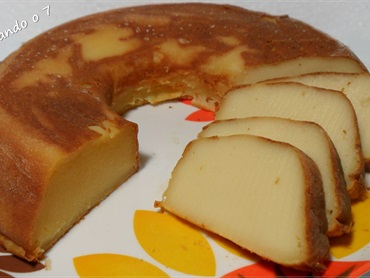
\includegraphics[width=0.4 \textwidth]{bolo.jpg}
    \caption{Foto do bolo.}
    \label{fig_do_bolo}
  \end{center}
\end{figure}

Uma das características mais marcantes do baeta é que a massa não leva fermento~\cite{Chavent:2003}, o que lhe confere um aspecto úmido e textura consistente levemente parecida à do pudim. Além do leite, que pode ser de origem animal (vaca), vegetal (coco) ou mista, os ingredientes de base incluem ovos, manteiga, farinha de trigo e açúcar~\cite{Saporta:1990}.

No livro História da alimentação no Brasil~\cite{Diday:1982}, de 1868, do escritor e historiador Câmara Cascudo, encontra-se a seguinte descrição:

\begin{center}
  \textit{Bolo Baeta: seis ovos com claras, uma quarta de manteiga (120 grs.), meia libra de açúcar (250 grs.), meia de farinha de trigo, leite de dois cocos, sumo de limão. Batem-se os ovos com o açúcar, depois o leite de coco com a manteiga e por último a farinha~\cite{Bock:1978}. Algumas receitas incluíam erva-doce e passas de uvas~\cite{Neto:2010}, sem os caroços. Fogo brando e lento. Forma redonda, previamente untada de manteiga. Era tradicional para o chá.}
\end{center}

Às vezes, também recebe~\cite{Diday:1991} a denominação de \textbf{bolo baieta} ou mesmo \textbf{bolo de leite}, já que leva muito desse ingrediente na receita tradicional.

\subsection{Receita de Bolo Baeta}

Bolo de Leite~\cite{Roque:2007}, Bolo Baeta, Engorda marido~\cite{Afonso:2004}, Bolo Ligado, varia de região o nome a ser chamado tudo resulta nesse bolo delicioso muito consumido aqui no Nordeste, Tem ligeiramente o aspecto de Pudim, bom-bocado de Padaria. Uma maravilha para acompanhar bons papos e uma xícara de café quente. É sempre um prazer você aqui prestigiando o Teretetê na cozinha

\subsection{Ingredientes}

\begin{itemize}
  \item $4$ ovos;
  \item $2$ e $1/2$ colheres de sopa de manteiga;
  \item $2$ e $1/2$ xícaras de açúcar;
  \item $3$ xícaras de farinha de trigo;
  \item $1$ litro de leite;
  \item Queijo ralado a gosto (Queijo coalho, queijo parmesão).
\end{itemize}

\subsection{Mode de Fazer}

Coloquem no liquidificador os ovos, a manteiga~\cite{Zisserman:2012}, o açúcar e bata por 3 a 4 minutos os ingredientes no liquidificador depois acrescentem o leite e a farinha e o queijo bata ate misturar despeje na forma untada de polvilhada e leve ao forno para assar por 50 a 60 minutos.

\section{Tabela Nutricional}

Podemos verificar os valores~\cite{Tamura:1978} nutricionais do bolo baeta na Tabela~\ref{tab_nutri}. Na Tabela~\ref{tab_vitaminas} é listado todas as vitaminas do bolo baeta.

\begin {table}[h!]
\begin{center}
\begin{tabular}{p{3.2cm}c}
\hline
Açúcar     & 16 mg  \\ \hline
Cálcio     & 166 mg  \\ \hline
Ferro      & 166 mg  \\ \hline
Potassio   & 166 mg  \\ \hline 
Sodio      & 166 mg  \\ \hline
Gorduras   & 166 mg  \\ \hline
\end{tabular}
\caption {Tabela Nutricional}
\label{tab_nutri} 
\end{center}
\end{table}

\begin {table}[h!]
\begin{center}
\begin{tabular}{|c|c|}
\hline
Vitamina A & 166 mg  \\ \hline
Vitamina K & 166 mg  \\ \hline
Vitamina C & 166 mg  \\ \hline
\end{tabular}
\caption {Tabela de Vitaminas}
\label{tab_vitaminas} 
\end{center}
\end{table}

\section{Demonstração matematica do Bolo Baeta}

$c^{2}=a^{2}+b^{2}$

\begin{displaymath}
  c^{2}=a^{2}+b^{2}
\end{displaymath}

\begin{displaymath}
\lim_{n \to \infty}
\sum_{k=1}^n \frac{1}{k^2}
= \frac{\pi^2}{6}
\end{displaymath}

Verificando a equação : $\lim_{n \to \infty}
\sum_{k=1}^n \frac{1}{k^2}
= \frac{\pi^2}{6}$

\begin{displaymath}
\sum_{i=1}^{n} \qquad
\int_{0}^{\frac{\pi}{2}} \qquad
\prod_\epsilon
\end{displaymath}

\begin{displaymath}
1 + \left( \frac{1}{ 1-x^{2} }
\right) ^3
\end{displaymath}

$\Big( (x+1) (x-1) \Big) ^{2}$\\
$\big(\Big(\bigg(\Bigg($\quad
$\big\}\Big\}\bigg\}\Bigg\}$\quad
$\big\|\Big\|\bigg\|\Bigg\|$

\begin{displaymath}
x_{1},\ldots,x_{n} \qquad
x_{1}+\cdots+x_{n}
\end{displaymath}

\begin{displaymath}
\mathbf{X} =
\left( \begin{array}{ccc}
x_{11} & x_{12} & \ldots \\
x_{21} & x_{22} & \ldots \\
\vdots & \vdots & \ddots
\end{array} \right)
\end{displaymath}

\begin{eqnarray}
f(x) &=& \cos x \\
f'(x) &=& -\sin x \\
\int_{0}^{x} f(y)dy &=& \sin x
\end{eqnarray}

\begin{displaymath}
\mathop{\mathrm{corr}}(X,Y)=
\frac{\displaystyle
\sum_{i=1}^n(x_i-\overline x)
(y_i-\overline y)}
{\displaystyle\biggl[
\sum_{i=1}^n(x_i-\overline x)^2
\sum_{i=1}^n(y_i-\overline y)^2
\biggr]^{1/2}}
\end{displaymath}

\begin{eqnarray}
\lefteqn{ \cos x = 1
-\frac{x^{2}}{2!} +{} }
\nonumber\\
& & {}+\frac{x^{4}}{4!}
-\frac{x^{6}}{6!}+{}\cdots
\end{eqnarray}

Teste teste teste Teste teste teste Teste teste teste Teste teste teste Teste teste teste \cite{Pressman:2007}

\bibliographystyle{acm}
\bibliography{BibDesk}

\end{document}

\end{document}
